\documentclass{beamer}

\usepackage[utf8]{inputenc}
\usepackage[T2A]{fontenc}
\usepackage[utf8]{inputenc}
\usepackage[russian]{babel}

% \usetheme{Berlin}

\addtobeamertemplate{navigation symbols}{}{%
    \usebeamerfont{footline}%
    \usebeamercolor[fg]{footline}%
    \hspace{1em}%
    \insertframenumber/\inserttotalframenumber
}

\title{Защищенное распределенное умножение матриц с использованием полиномиального кодирования}
\author{Авдотьин Е., Глинский К., Ендовицкий Е.}
\institute{МФТИ}
\date{2019}

\begin{document}
    
    \frame{\titlepage}

    \begin{frame}
        \frametitle{Постановка задачи}
        \begin{itemize}
            \item<1-> \textbf{Клиент}
            \begin{itemize}
                \item Имеет две матрицы: $A \in \mathbb{F}_q^{r\times s}$, $B \in \mathbb{F}_q^{s\times t}$
                \item Хочет получить матрицу $C = AB \in \mathbb{F}_q^{r \times t}$
            \end{itemize}
            \item<2-> \textbf{Серверы}
            \begin{itemize}
                \item Каждый может получать на вход две матрицы и вычислять их произведение
            \end{itemize}
            \item<3-> \textbf{Цель}
            \begin{itemize}
                \item Вычислить $C = AB$ с использованием серверов, при этом ни один из них не должен иметь информацию об $A$ и $B$
                % \item 
            \end{itemize}
        \end{itemize}
    \end{frame}

    \begin{frame}
        \frametitle{Полиномиальное кодирование: пример}
        \begin{itemize}
            \item Имеется две матрицы $A \in \mathbb{F}_q^{r\times s}$, $B \in \mathbb{F}_q^{s\times t}$
            \begin{itemize}
                \item<1-> Сгенерируем две случайные матрицы $R \in \mathbb{F}_q^{r\times s}$, $S \in \mathbb{F}_q^{s\times t}$
                \item<2-> Рассмотрим многочлены
                \begin{equation*}
                    f(x) = A + Rx, \; g(x) = B + Sx
                \end{equation*}
                \item<3-> Их произведение имеет вид
                \begin{equation*}
                    h(x) = f(x) \cdot g(x) = AB + \left(AS + RB\right) + RSx^2
                \end{equation*}
                \item<4-> Имея 3 значения $h$, можно восстановить многочлен $h(x)$ и найти $h(0) = AB$
            \end{itemize}
        \end{itemize}
    \end{frame}

    \begin{frame}

        \frametitle{Распределенное полиномиальное кодирование}
        \begin{itemize}
            \item Вычисление значений $h(x)$ может производиться на распределенных серверах
            \begin{figure}[t!]
                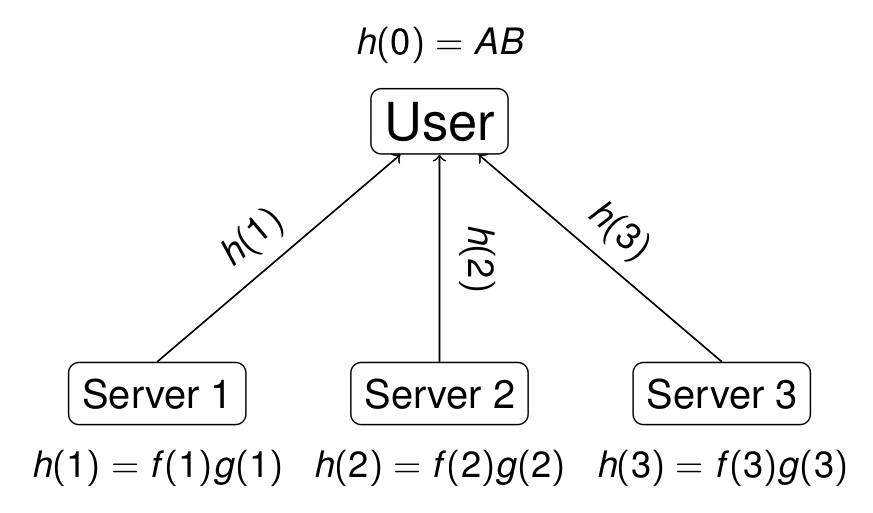
\includegraphics[width=0.8\textwidth]{poly_code.png}
            \end{figure}
            \item $f(x) = A + Rx$
            \item $g(x) = B + Sx$
            \item $h(x) = f(x) \cdot g(x) = AB + \left(AS + RB\right) + RSx^2$
        \end{itemize}
        
    \end{frame}

    \begin{frame}
        
        \frametitle{Разбиение матриц}
        Рассмотрим разбиение матриц:
        \begin{itemize}
            \item<1-> Первого множителя -- по строкам
            \begin{equation*}
                A = 
                \begin{bmatrix}
                    A_1 \\ \vdots \\ A_K
                \end{bmatrix}
            \end{equation*}
            \item<2-> А второго -- по столбцам
            \begin{equation*}
                B = 
                \begin{bmatrix}
                    B_1 & \dots & B_L
                \end{bmatrix}
            \end{equation*}
            \item<3-> Их произведение будет иметь вид
            \begin{equation*}
                AB =
                \begin{bmatrix}
                    A_1B_1 & \dots & A_1B_L \\
                    \vdots & \ddots & \vdots \\
                    A_K B_1 & \dots & A_K B_L
                \end{bmatrix}
            \end{equation*}
            \end{itemize}
    \end{frame}

\end{document}